%%%%%%%%%%%%%%%%%%%%%%%
%%      Lecon 1      %%
%%%%%%%%%%%%%%%%%%%%%%%

\chapter{Les origines de la crise : \\ Les prêts hypothécaires "subprimes"}
Comme beaucoup le savent, un prêt hypothécaire est un prêt accordé pour un bien immobilier en garantissant le remboursement par ce bien. En effet, en cas d'impossibilité de remboursement, la banque met la main sur le bien. C'est sur le terme "subprime" que nous allons nous intéressé dans ce chapitre qui sera expliqué dans son contexte.

\section{Ca craque une première fois}
\textbf{Ralph Cioffi} est un gestionnaire "génial" de fonds. Il collecte beaucoup d'argent chez les investisseurs et investit cet argent dans des actifs (actions, immeubles, ...). Puisqu'un gestionnaire de fond est rémunéré selon les montants gérés et sur la rentabilité, il s'efforce d'obtenir le meilleur rendement (retour d'argent) avec un risque faible (peu d'argent). Pour améliorer ce rendement, \textbf{on s'endette au maximum !} \\
D'un autre côté, les banques qui prêtent veulent être sûres de retrouver leur mise \footnote{La banque \textbf{Merrill Lynch} a prêté beaucoup d'argent au fonds géré par Ralph Cioffi.}. Pour cela, elles vérifient régulièrement si la valeur des actifs est supérieure aux dettes. Si ce n'est pas le cas, elle procède à un \textbf{appel de marge} (demande de l'argent au fonds). \\

Pour financer l'appel de marge, on a, dans l'ordre, trois chances :
\begin{enumerate}
\item \textbf{Utiliser le cash disponible dans le fonds.}
\item \textbf{Faire appel aux investisseurs.}
\item \textbf{Vendre des actifs.}
\end{enumerate}

Ce qui s'est passé en 2007, c'est que justement il n'y avait plus de cash, les investisseurs refusaient d'investir et les biens ne se vendaient pas ! De ce fait, les fonds étaient virtuellement en faillite. \\

\section{Les subprimes}
Mais comment en est-on arrivé à avoir des actifs invendables ? C'est à cause des financiers : 

\begin{enumerate}
\item \textbf{La Finance est modélisée}\\
On était capable de mettre tous les risques en équation et donc on pensait les contrôler. 

\item \textbf{La Finance n'est pas régulée}\\
On prêtait et empruntait sans trop de difficultés et sans règles.

\item \textbf{La Finance est organisée pour prêter le plus possible}\\
Si on a du cash, au plus on prête, au plus le \textbf{bonus} (grâce aux intérêts) sera élevé. Donc on prêtait à tout le monde, qu'il soit CEO \footnote{Chief Executive Officer.} ou employé de guichet.
\end{enumerate}
 
On prêtait donc à presque tout le monde pour acquérir un logement et c'est ce que l'on appelle les \textbf{subprimes}. Ce système fait plaisir aux individus mais aussi à l'économie (l'économie tourne). Les financiers avaient pour hypothèse que \textbf{le prix de l'immobilier ne cesserait d'augmenter quoiqu'il se passe}. Et bein quand c'est le contraire qui s'est passé, ça a fait mal.

\section{Comparaison des différents systèmes de prêt}
Une comparaison entre les différents prêt hypothécaires est disponible à partir du \textbf{slide 8} dans le cours mais voici un bref résumé :

\begin{itemize}
\item \textbf{Prêt hypothécaire classique (taux fixe)}\\
La banque ne prête que 80 \% de la valeur du bien, les 20 \% devant être un apport personnel. Pour un taux fixe et un revenu de ménage mensuel moyen (2700 euro), le ménage devra rembourser environ 47 \% de son salaire mensuel, ce qui est assez lourd. Mais si le salaire monte (3400 euro), on peut diminuer à 38 \%. 

\item \textbf{Prêt hypothécaire à taux variable}\\
Dans les mêmes conditions, le taux qui est plus faible que le fixe à la base peut soit augmenter, soit diminuer. Dans le cas où le taux diminue, c'est plus avantageux au niveau du remboursement. Par contre dans le cas où le taux augmente, on se fait avoir. C'est pire si le salaire moyen n'augmente pas après quelques années et je ne parle même pas du cas où le salaire diminuerai ! Aujourd'hui, les taux sont tellement bas qu'il est préférable de prendre un taux fixe.

\item \textbf{Prêt hypothécaire aux USA (taux variable et pas de limite à la quote part des revenus)}\\
Dans ce modèle, la banque prête la totalité de la valeur du bien. Si le taux augmente avec le temps et que le salaire reste inchangé, la part de remboursement commence aux environ de 65 \% et peut atteindre jusque 92 \%. Il y a donc un réel risque de \textbf{faillite personnel} dans ce système !

\item \textbf{Prêt hypothécaire aux USA (Quotité de 120 \% et "Negative amortization")}\\
Dans ce modèle la banque va non seuelement prêter la totalité de la somme, mais elle donne aussi 20 \% de cash en plus pour usage personnel (trop d'osey). De plus, pendant 5 ans le client ne devra rembourser que les intérêt (remboursement faible) ce qui donne un remboursement d'à peu près 50 \% du salaire. Cependant, après ces 5 ans, quand on commence à payer tout le prêt, si on a de la chance et que le salaire augmente, on aura un remboursement d'environ 80 \%. Si le salaire reste fixe ou qu'il diminue, alors on peut faire ses prières parce qu'on dépassera les 100 \% !
\end{itemize}


\section{Risque considéré comme faible par les banquiers}
Puisqu'on prête plus, le banquier aura plus de comission et sera gagnant. Celui qui emprunte pourra consommer plus et ainsi doper l'économie tout en étant propriétaire de logement. \\
Comme précisé plus haut, les banquiers font l'hypothèse que le prix de l'immobilier ne fera qu'augmenter. Si jamais il y a des problèmes, ce n'est pas grâve puisqu'ils récupère le bien et se fait encore plus d'argent en la revendant.\\

\begin{center}
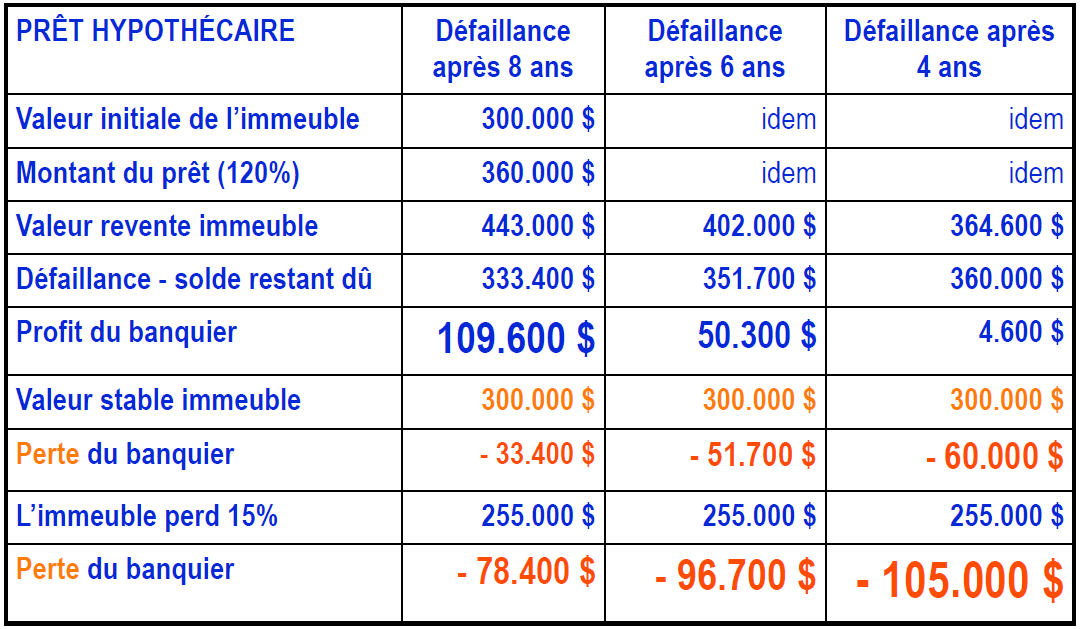
\includegraphics[scale=0.4]{1}
\end{center}

Sur la figure ci-dessus, on peut voir que le banquier gagne d'autant plus que la défaillance arrive tard. Bien sûr, ce n'est le cas que lorsque les prix montent. En effet, si la valeur du bien reste constant, le banquier perd d'office de l'argent (puisqu'il prête 120 \%). Si jamais la valeur du bien diminue, c'est la dégringolade.
